%\title{LaTeX Portrait Poster Template}
%%%%%%%%%%%%%%%%%%%%%%%%%%%%%%%%%%%%%%%%%
% a0poster Portrait Poster
% LaTeX Template
% Version 1.0 (22/06/13)
%
% The a0poster class was created by:
% Gerlinde Kettl and Matthias Weiser (tex@kettl.de)
% 
% This template has been downloaded from:
% http://www.LaTeXTemplates.com
%
% License:
% CC BY-NC-SA 3.0 (http://creativecommons.org/licenses/by-nc-sa/3.0/)
%
%%%%%%%%%%%%%%%%%%%%%%%%%%%%%%%%%%%%%%%%%

%----------------------------------------------------------------------------------------
%	PACKAGES AND OTHER DOCUMENT CONFIGURATIONS
%----------------------------------------------------------------------------------------

\documentclass[a0,portrait]{a0poster}

\usepackage{multicol} % This is so we can have multiple columns of text side-by-side
\columnsep=100pt % This is the amount of white space between the columns in the poster
\columnseprule=3pt % This is the thickness of the black line between the columns in the poster

\usepackage[svgnames]{xcolor} % Specify colors by their 'svgnames', for a full list of all colors available see here: http://www.latextemplates.com/svgnames-colors

\usepackage{times} % Use the times font
%\usepackage{palatino} % Uncomment to use the Palatino font

\usepackage{graphicx} % Required for including images
\graphicspath{{figures/}} % Location of the graphics files
\usepackage{booktabs} % Top and bottom rules for table
\usepackage[font=small,labelfont=bf]{caption} % Required for specifying captions to tables and figures
\usepackage{amsfonts, amsmath, amsthm, amssymb} % For math fonts, symbols and environments
\usepackage{wrapfig} % Allows wrapping text around tables and figures
\usepackage{capt-of}
\usepackage{multirow}
\usepackage{bbold}
\usepackage{wrapfig}

\begin{document}

%----------------------------------------------------------------------------------------
%	POSTER HEADER 
%----------------------------------------------------------------------------------------

% The header is divided into two boxes:
% The first is 75% wide and houses the title, subtitle, names, university/organization and contact information
% The second is 25% wide and houses a logo for your university/organization or a photo of you
% The widths of these boxes can be easily edited to accommodate your content as you see fit

\begin{minipage}[b]{0.75\linewidth}
\VeryHuge \color{NavyBlue} \textbf{Probing Neural Network Comprehension \\
of Natural Language Arguments} \color{Black}\\[0.5cm] % Title
\huge \textbf{Timothy Niven} and \textbf{Hung-Yu Kao}\\[0.5cm] % Author(s)
\huge 
Intelligent Knowledge Management Lab \\[0.5cm]
National Cheng Kung University, Taiwan\\[0.4cm] % University/organization
\Large \texttt{tim.niven.public@gmail.com}\\
\end{minipage}
%
\begin{minipage}[b]{0.25\linewidth}

\includegraphics[width=17.5cm]{NCKU_Logo_2011.png}
\end{minipage}

\vspace{1cm} % A bit of extra whitespace between the header and poster content

%----------------------------------------------------------------------------------------

\begin{multicols}{2} % This is how many columns your poster will be broken into, a portrait poster is generally split into 2 columns

\large

\section*{How do you know two sentences connect argumentatively?}

\vspace{8pt}

\begin{center}
  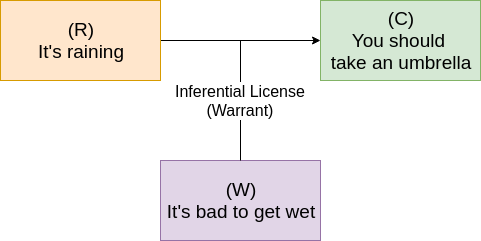
\includegraphics[width=0.5\linewidth]{rain-umbrella-single.png}
\end{center}

\vspace{8pt}

\begin{itemize}
    \item Warrants provide a basis for making these connections
    \item Would have to \textit{learn} and \textit{reason} with warrants
\end{itemize}

\section*{Even supplying warrants, reasoning with them is very hard}

\vspace{8pt}

\begin{center}
  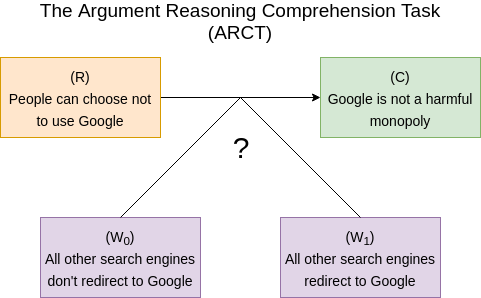
\includegraphics[width=0.45\linewidth]{google.png}
  \hspace*{0.09\linewidth}
  \includegraphics[width=0.35\linewidth]{ARCT_ARCHITECTURE.png}
\end{center}

\begin{align*}
    R \land W_0 &\rightarrow C \\
    R \land W_1 &\rightarrow \lnot C \\
\end{align*}

\vspace{8pt}

\begin{itemize}
    \item Binary classification with a small dataset (1,210 training data points)
    \item SemEval 2018 shared task systems found it hard to break 60\% accuracy
    \item Still need significant world knowledge: how do web directs relate to the concept of monopoly in the context of search engines?
\end{itemize}

\section*{BERT is a strong learner}

\vspace{8pt}

\begin{center}
  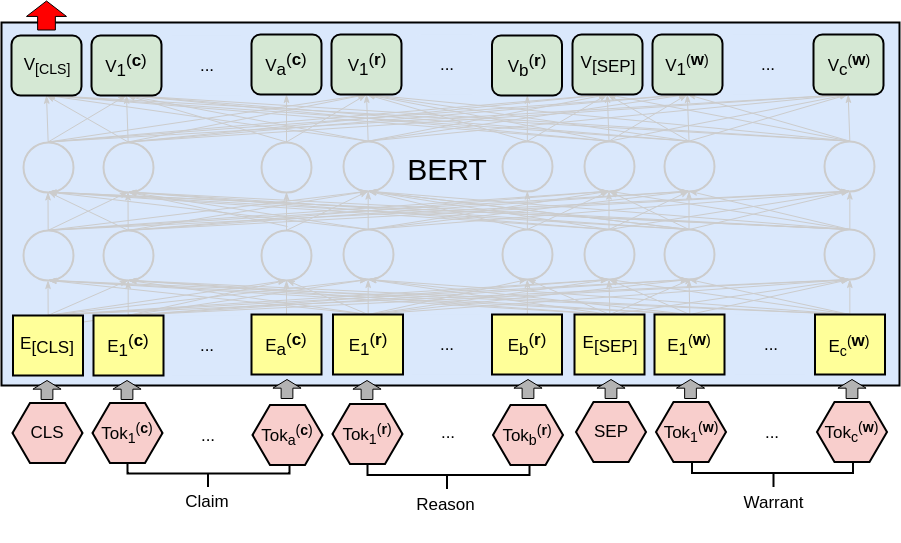
\includegraphics[width=0.8\linewidth]{BERT_ARCT.png}
\end{center}

\begin{center}
\begin{tabular}{|l|c|ccc|}
\hline
\multirow{2}{*}{} & \multicolumn{1}{c|}{\textbf{Dev}} & \multicolumn{3}{c|}{\textbf{Test}} \\
& Mean & Mean & Median & Max \\
\hline
Human (trained) & & 0.909 $\pm$ 0.11 &  &  \\
Human (untrained) & & 0.798 $\pm$ 0.16 & &  \\
BERT (Large) & 0.701 $\pm$ 0.05 & 0.671 $\pm$ 0.09 & \textbf{0.712} & \textbf{0.770} \\
Choi and Lee (2018) & \textbf{0.716} $\pm$ 0.01 & \textbf{0.711} $\pm$ 0.01 & &  \\
BERT (Base) & 0.680 $\pm$ 0.02 & 0.623 $\pm$ 0.07 & 0.651 & 0.685 \\
Botschen et al. (2018) & 0.674 $\pm$ 0.01 & 0.568 $\pm$ 0.03 & & 0.610 \\
BoV & 0.639 $\pm$ 0.02 & 0.564 $\pm$ 0.02 & 0.569 & 0.595 \\
BiLSTM & 0.658 $\pm$ 0.01 & 0.552 $\pm$ 0.02 & 0.552 & 0.592 \\
\hline
\end{tabular}
\end{center}

\vspace{16pt}

\begin{itemize}
    \item 5/20 BERT Large runs were degenerate - non-skewed mean is $0.716 \pm 0.04$
    \item BERT's maximum performance of 77\% is three points behind the average (untrained) human baseline
    \item But this does not seem reasonable since BERT lacks the required knowledge
    \item What has BERT learned?
\end{itemize}

\section*{There are spurious statistical signals in the dataset}

\begin{minipage}{.5\linewidth}
    \begin{itemize}
        \item Let $k$ be some heuristic, such as a unigram or bigram
        \item $\mathbb{T}_j^{(i)}$ is the set of tokens in warrant $j$
        \item $y^{(i)} \in \{0, 1\}$ is the label
    \end{itemize}
\end{minipage}
\begin{minipage}{.5\linewidth}
    \begin{flushright}
        \begin{center}
        \begin{tabular}{|l|cc|}
        \hline
         $k =$ \textbf{``not''} & \textbf{Productivity} & \textbf{Coverage} \\
        \hline
        \textbf{Train} & 0.65 & 0.66 \\
        \textbf{Validation} & 0.62 & 0.44 \\
        \textbf{Test} & 0.52 & 0.77 \\
        \hline
        \textbf{All} & \textbf{0.61} & \textbf{0.64} \\
        \hline
        \end{tabular}
        \end{center}
    \end{flushright}
\end{minipage}

\vspace{8pt}

\begin{center}
    \begin{align*}
        \alpha_k &= \sum_{i=1}^n \mathbb{1} \left[ \exists j, k \in \mathbb{T}^{(i)}_j \land k \notin \mathbb{T}^{(i)}_{\lnot j} \right] \\
        \text{productivity} &= \frac{\sum_{i=1}^n \mathbb{1} \left[ \exists j, k \in \mathbb{T}^{(i)}_j \land k \notin \mathbb{T}^{(i)}_{\lnot j} \land y^{(i)} = j \right]}{\alpha_k} \\
        \text{coverage} &= \frac{\alpha_k}{n}
    \end{align*}
\end{center}

\vspace{8pt}

\begin{itemize}
    \item \textit{Productivity} measures how often you are rewarded for relying on a cue
    \item \textit{Coverage} measures how strong the signal is in the data
    \item The strongest cue is ``not''
    \item A great many more exist, albeit at much lower productivity for any decent coverage
\end{itemize}

\section*{All models exploit these spurious statistics; BERT best of all}

\begin{center}
\small
\begin{tabular}{|l|ccc|}
\hline
\multirow{2}{*}{} & \multicolumn{3}{c|}{\textbf{Test}} \\
& \textbf{Mean} & \textbf{Median} & \textbf{Max} \\
\hline
BERT & \textbf{0.671} $\pm$ 0.09 & \textbf{0.712} & \textbf{0.770} \\
BERT (W) & 0.656 $\pm$ 0.05 & 0.675 & 0.712 \\
BERT (R, W) & 0.600 $\pm$ 0.10 & 0.574 & 0.750 \\
BERT (C, W) & 0.532 $\pm$ 0.09 & 0.503 & 0.732 \\
\hline
BoV & 0.564 $\pm$ 0.02 & 0.569 & 0.595 \\
BoV (W) & 0.567 $\pm$ 0.02 & 0.572 & 0.606 \\
BoV (R, W) & 0.554 $\pm$ 0.02 & 0.557 & 0.579 \\
BoV (C, W) & 0.545 $\pm$ 0.02 & 0.544 & 0.589 \\
\hline
BiLSTM & 0.552 $\pm$ 0.02 & 0.552 & 0.592 \\
BiLSTM (W) & 0.550 $\pm$ 0.02 & 0.547 & 0.577 \\
BiLSTM (R, W) & 0.547 $\pm$ 0.02 & 0.551 & 0.577 \\
BiLSTM (C, W) & 0.552 $\pm$ 0.02 & 0.550 & 0.601 \\
\hline
\end{tabular}
\end{center}

\vspace{8pt}

\begin{itemize}
    \item (W) just considers warrants (like a hypothesis-only NLI baseline)
    \item (R, W) additionally considers the reason
    \item (C, W) considers the claim and warrant
    \item Each of these setups breaks the task and reflects learning of spurious statistics
    \item The entirety of BERT's best 77\% can be accounted for by these degenerate setups
\end{itemize}

\section*{We can eliminate the main problem in the dataset}

\vspace{8pt}

\begin{center}
  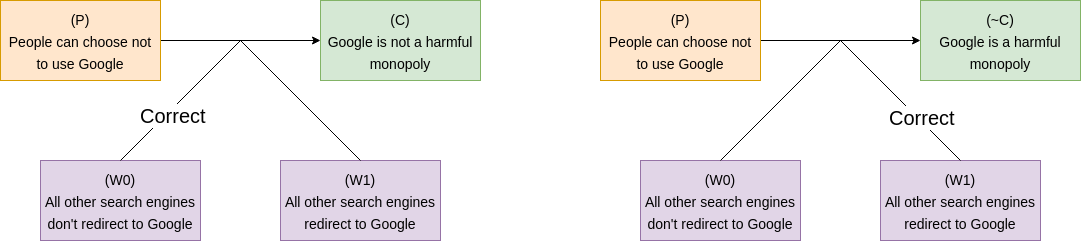
\includegraphics[width=0.8\linewidth]{adversarial-data.png}
\end{center}

\vspace{8pt}

\begin{itemize}
    \item We create adversarial examples by negating each claim and flipping the label
    \item The major source of spurious signal is eliminated by mirroring around the labels
\end{itemize}

\section*{The new state of the art is random}

\vspace{8pt}

\begin{center}
\begin{tabular}{|l|ccc|}
\hline
\multirow{2}{*}{} & \multicolumn{3}{c|}{\textbf{Test}} \\
& \textbf{Mean} & \textbf{Median} & \textbf{Max} \\
\hline
BERT & \textbf{0.504} $\pm$ 0.01 & \textbf{0.505} & \textbf{0.533} \\
BERT (W) & 0.501 $\pm$ 0.00 & 0.501 & 0.502 \\
BERT (R, W) & 0.500 $\pm$ 0.00 & 0.500 & 0.502 \\
BERT (C, W) & 0.501 $\pm$ 0.01 & 0.500 & 0.518 \\
\hline
\end{tabular}
\end{center}

\section*{Conclusion}

\vspace{8pt}

\begin{itemize}
    \item ARCT remains very difficult
    \item The adversarial dataset should be the standard in future work
    \item BERT is a strong learner capable of picking up on very subtle statistical cues
    \item As our models get stronger, the issue of spurious statistics becomes more pressing
\end{itemize}

\end{multicols}
\end{document}